% Created 2023-02-02 Thu 09:59
\documentclass[9pt, b5paper]{article}
\usepackage{xeCJK}
\usepackage{minted}
\usepackage[T1]{fontenc}
\usepackage[scaled]{beraserif}
\usepackage[scaled]{berasans}
\usepackage[scaled]{beramono}
\usepackage{graphicx}
\usepackage{xcolor}
\usepackage{multirow}
\usepackage{multicol}
\usepackage{float}
\usepackage{textcomp}
\usepackage{algorithm}
\usepackage{algorithmic}
\usepackage{latexsym}
\usepackage{natbib}
\usepackage{geometry}
\geometry{left=1.2cm,right=1.2cm,top=1.5cm,bottom=1.2cm}
\newminted{common-lisp}{fontsize=\footnotesize} 
\usepackage[xetex,colorlinks=true,CJKbookmarks=true,linkcolor=blue,urlcolor=blue,menucolor=blue]{hyperref}
\author{deepwaterooo}
\date{\today}
\title{ET}
\hypersetup{
  pdfkeywords={},
  pdfsubject={},
  pdfcreator={Emacs 27.2 (Org mode 8.2.7c)}}
\begin{document}

\maketitle
\tableofcontents


\section{ET框架框架设计模块功能等}
\label{sec-1}
\subsection{一个双端框架的12个项目,目录结构}
\label{sec-1-1}
\begin{itemize}
\item 就不知道这12个项目是如何组织构建起来的
\end{itemize}
\subsubsection{客户端的四个项目}
\label{sec-1-1-1}

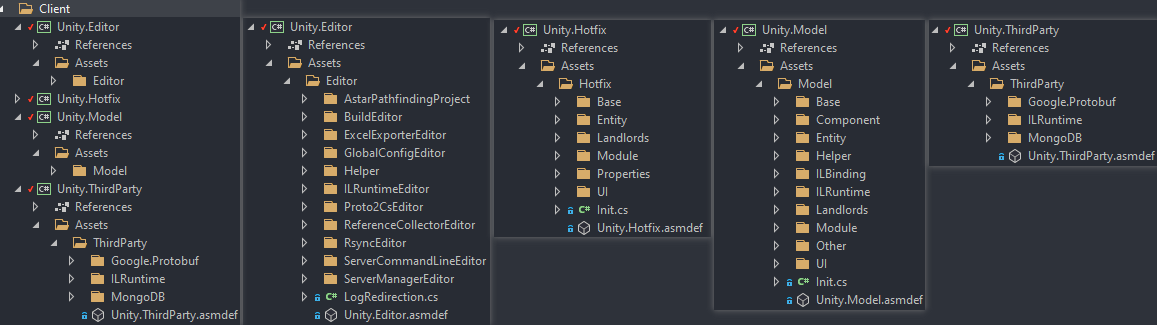
\includegraphics[width=.9\linewidth]{./pic/readme_20230201_200218.png}
\subsubsection{服务器端的8个项目:}
\label{sec-1-1-2}

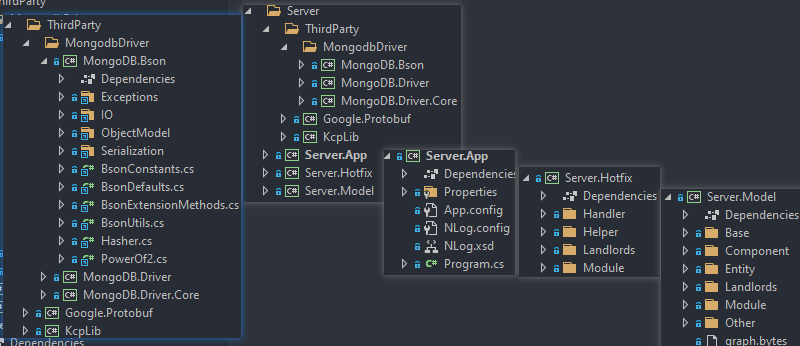
\includegraphics[width=.9\linewidth]{./pic/readme_20230201_201117.png}
\subsection{模块功能管理}
\label{sec-1-2}
\subsubsection{ET框架中事件使用的规则和注意事项}
\label{sec-1-2-1}
\begin{itemize}
\item \textbf{事件结构体的定义} 必须在Model或ModelView下, \textbf{事件的订阅和发布} 必须在Hotfix或HotfixView下 (是否为View层根据是否需要UnityAPI决定)
\item 在ET框架中 \textbf{View层可以直接调用逻辑层的代码} ,而 \textbf{逻辑层不允许直接调用View层的代码} ,所以逻辑层想要和View层交互只能使用抛出事件的方式,让View层进行订阅进行相应的处理。
\end{itemize}
\subsubsection{ET框架下ETTask的异步编程}
\label{sec-1-2-2}
\begin{itemize}
\item 开发早期都是使用协程或者多线程进行程序异步的实现,
\item 在C\#5.0之后引入了Tasync await等关键字可以轻松优美的实现程序的异步进行。
\item Task是C\#异步编程库的异步功能基础类型,包含了多线程的使用。
\item 而ET框架主打的是 \textbf{多进程单线程} ,所以使用ETTask对Task进行了封装,使其不用考虑多线程的共享难题,更易于使用。
\end{itemize}
\subsubsection{协程}
\label{sec-1-2-3}
\begin{itemize}
\item 协程其实就是创建一段程序辅助主线程的运行,注意 \textbf{协程不是多线程,其仍运行在主线程当中,其只是将一个函数按照一定的条件分解成若干块,穿插在主线程的各个位置中运行。}
\item async 和 await关键字
\begin{itemize}
\item async是修饰函数的关键字,被修饰的函数称为异步函数,只有被此关键字修饰的函数才能使用await关键字
\item await关键字后跟一些表达式(一般是返回值为ETTask的函数),在异步函数运行到此时会立即跳出函数,继续执行原逻辑。
\item await返回前会做出保证,保证await后表达式的任务完成后,执行点会跳回异步函数中,继续向后执行剩余代码
\item 若await后表达式正常返回,可用变量接收表达式的返回值,表达式的返回值类型为定义表达式ETTask<>的泛型
\end{itemize}
\end{itemize}

\section{小小服务器:要怎么才能开始动手试图去实现这个小服务器呢?}
\label{sec-2}
\subsection{如果适配ET框架,现游戏可能哪些模块版块存在问题}
\label{sec-2-1}
\begin{itemize}
\item 我也觉得ET框架可能不太适合我现在的游戏(也就是说,把我的游戏完全适配成ET框架来开发,原本只需要一个小小服务器,完全适配为ET框架,就把问题弄得狠复杂了。。。),
\item 使用ET框架,我所有的安卓基础就会被抛到九宵去外,不再关安卓SDK  NDK什么事儿了。。。。。是对自己太大的损耗。而我原本还可以简单封装实现的安卓录屏,游戏内使用安卓SDK相关功能模块录屏游戏过程等,会被全部废掉,损失太大不值得。我觉得我就只要个文件服务器加个数据库而已。
\item 原因是:我现在还想不通若是用ET框架来实现自己游戏的(服务器与客户端双端都可以热更新),我该如何实现我的方块砖10个按钮上的点击事件,射线检测?它的ILRuntime热更新程序域里对射线检测包的组件安装可能会成为自己狠大的问题,因为还不是狠懂里面的内部原理.这个模块重构的原理是:把射线检测,如果必要一定要,封装成如ET中任何其它可装载卸载的组件一样的装载到某个必要场景上去.
\begin{itemize}
\item ET里有个检测鼠标左右键位置的帮助类,但跟射线检测应该还是相差狠远的.而游戏场景里面有一个OperaCompoent,这个组件会实时监听按键的点击并且将点击的位置发送给服务器,服务器再传送回客户端
\end{itemize}
\item 所以,现在对这个框架,最深的感触是:盲人摸象,摸每部分细节似乎都快清楚了,却无法组装从一个更高的层面上来理解和把握框架设计,无法吃透,在大框架功能模块上犯难,在网上再搜一搜
\item 我可以把两组按钮画面同样做成预设与热更新资源包,射线检测同样会成为可装载可卸载的组件,可是再后面射线检测到的物体逻辑,感觉有点儿复杂了
\item 
\end{itemize}
\subsection{如果不适配,怎么弄个服务器带数据库等逻辑?}
\label{sec-2-2}
\begin{itemize}
\item 使用部分共享源码的双端(共享的是文件服务器8个项目,MongoDB数据库服务器, Realm注册登录用,网关服,Location服, ETTAsk, RPC消息机制, NetComponent等自己机对陌生需要练习,而自己的服务器也不可缺省的相关功能)
\item 现在知道自己整的不沦不类的服务器所谓的登录,登录的是网页上的认证相关,跟自己真正要实现的游戏里注册登录服保存数据库完全两回事,现在知道了。
\item 作用ET的头,实现用户注册与登录,适配自己现有游戏的尾,游戏除了入口之外全游戏进热更新程序域里
\item 那么自己的现框架架构作尾,全游戏逻辑进热更新域,存在的问题就变成是:
\item 我无法再实时动态检查用记上下线顶号之类的,我只能默认登录过就是登录状态,可是用户下线了,或更严格的说掉线了,服务器并不及时知道,可以通过安卓SDK中的按钮登出知道。但是掉网了掉线了呢?
\item 再则,ILRuntime热更新程序域里,我又该如何实现在热更新程序域里网络上载用户的游戏保存进展?这里需要去想和理解,为什么它ET框架就可以在热更新程序域里同网络交互,你哪里还没有想明白?
\item ET框架,热更新程序域里装载的组件,只是帮助与外界游戏程序域连通好,真正的网络请求上传下载等是在热更新域外面完成链接式传进去的?感觉对这个大框架没有掌握好,脑袋仍然是在像糊糊一样。。。
\item 各种泛型,接口的定义,一二三个参数等的泛型接口定义(你可以去找一找工程中的各种ILRuntime的适配器),全都是都可以成为热更新域里能够被游戏程序域里识别的原因,所以狠多设计,自带ILRuntime的适配性质
\item 那么就可以小一点儿一点儿地来,先弄个登录窗口,实现服务器的注册登录保存登录信息到数据库,相对比较小点儿的逻辑.这个过程中把MongoDB数据库的配置等所有连接过程中必要的步骤,可能出现的问题给解决掉,就算前进了一小步呀
\item 不知道怎么开始,也不知道怎么创建可以㠌套的像是安卓模块库一样的子工程,就只能把小游戏斗地主复制一份了再从它的基础上来改?!!!
\item 如果简单一点儿开始,我觉得我应该是可以先把简单点儿的MongoDB数据库连接成功,把用户登录相关的逻辑,网络交互的部分,ETTask RPC ACTOR消息等,哪怕是复制,把这部分弄过去
\end{itemize}
\subsection{ET框架}
\label{sec-2-3}
\begin{itemize}
\item \url{https://blog.csdn.net/qq_33574890/article/details/128244264?spm=1001.2101.3001.6650.1&utm_medium=distribute.pc_relevant.none-task-blog-2\%7Edefault\%7EAD_ESQUERY\%7Eyljh-1-128244264-blog-123841252.pc_relevant_multi_platform_whitelistv4&depth_1-utm_source=distribute.pc_relevant.none-task-blog-2\%7Edefault\%7EAD_ESQUERY\%7Eyljh-1-128244264-blog-123841252.pc_relevant_multi_platform_whitelistv4&utm_relevant_index=2} 上次看看得不是狠懂,这次再看,至少是觉得UI的逻辑处理,作者的观点更自然真实一些,放在一个文件一起处理,个人认为更好,而不是折分成为几个文件 
\begin{minted}[fontsize=\scriptsize,linenos=false]{csharp}
class LoginState:State{
	void OnEnter(){
		UI.Show()
	}
	void OnLeave(){
		UI.Hide()
	}
}
\end{minted}
\end{itemize}

\section{登录协议流程}
\label{sec-3}
\begin{itemize}
\item 因为登录协议是客户端与服务器通信的,不属于服务器内部协议,所以打开OuterMessage.proto,里面存放的都是客户端与服务器通信定义的协议数据。
\item 比如定义如下,登录协议:
\end{itemize}
\begin{minted}[fontsize=\scriptsize,linenos=false]{text}
message C2G_LoginGate // IRequest
{
	int32 RpcId = 90;
	int64 Key = 1;	// 帐号
}

message G2C_LoginGate // IResponse
{
	int32 RpcId = 90;
	int32 Error = 91;
	string Message = 92;
	int64 PlayerId = 1;
}
\end{minted}
\begin{itemize}
\item emacs里org-mode exporte-to-pdf希望有个latex选择可以自动将\^{}I转化为空格,而不是这种字符,晚点儿再弄这个
\item 注意点: \textbf{没有意识到像是注释一样的片段,这个协议里,会成为标注或是标签}
\begin{itemize}
\item 1.因为登录是请求-响应类型协议(即发送一条数据,并期望返回一条数据),所以注意对应C2R\_Login协议带有“//ResponseType R2C\_Login”标志,在生成协议时,用于标记这个C2R\_Login请求对应的响应类型为R2C\_Login
\item 2.因为请求是直接发送给realm服的,所以是普通的IRequest类型协议,标记为IRequest
\item 3.R2C\_Login回复类消息结构,因为是Realm服发送给客户端的,因此是一个普通IResponse
\item 4.注意两个协议类里面都有RpcId,主要用于发送请求-响应类消息时,发送将自己的RpcID发送出去,返回时带回这个值,用于发送方接受到返回协议时,可以找到对应的是哪一个请求协议返回来的。
\end{itemize}
\end{itemize}

\section{一步一步的进展 }
\label{sec-4}
\begin{itemize}
\item 首先,把斗地方大厅改写为游戏主菜单的三个选项
\end{itemize}

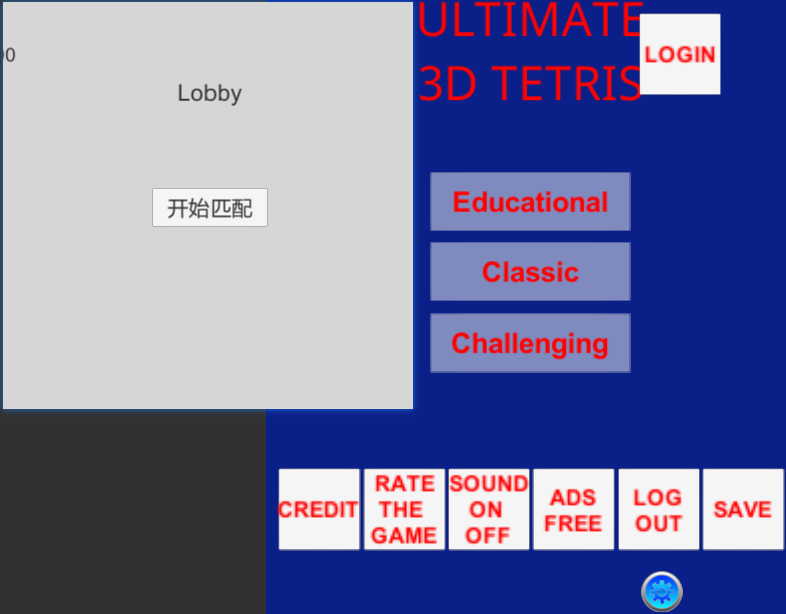
\includegraphics[width=.9\linewidth]{./pic/readme_20230201_202642.png}
\begin{itemize}
\item 把这个界面的相关上下文全部适配好:UI的自动创建生成系统,UI的按钮点击回调等
\item 这里想要找的是: 在点击的回调里如何,是否可以卸载装载UI组件,还是说必须得去HotfixView 什么视图层来处理这些逻辑呢?
\end{itemize}
\subsection{UIType.cs: 这种类型的定义好像不止加一个地方,一个地方不够,可是大的框架架构还是没搞明白}
\label{sec-4-1}
\begin{minted}[fontsize=\scriptsize,linenos=false]{csharp}
namespace ETHotfix {

    public static partial class UIType {
        public const string Root = "Root";
        public const string UILogin = "UILogin"; // 注册 登录 界面
        public const string UILobby = "UILobby"; // 主菜单 三选项

// 上面的界面远远不够呀。。。
        public const string UIEducationalMode = "UIEducationalMode"; 

        public const string UIEducational = "UIEducational"; 
 // 怎么再把它细化为:三 四 五方格呢? 应该是要用同一接口的不同实现,完全重复写三个系统会把人弄死的。。。。。
        public const string UIGridThree = "UIGridThree";
        public const string UIGridFour = "UIGridFour"; 
        public const string UIGridFive = "UIGridFive"; 

        // 那么就涉及游戏界面的折分:哪些是可以公用,哪些是不得不细化最小粒度的?
        
        public const string UIClassic = "UIClassic"; 

        public const string UIChallenge = "UIChallenge"; 
 // 挑战难度:要定义接口来实现20-50个不同的实现了?        
    }
}
\end{minted}

\begin{itemize}
\item 安卓SDK这个框架其实并不受影响。但本质是所有安卓SDK的东西不能够热更新。因为ET是网络多人游戏框架的,可能更多的是不适合添加与适配案桌SDK。这些晚点儿再得结论好了,反正我的案桌SDK本质也是可要可不要。如果能够快速掌握一个比较好的双端框架的话
\item 不知道若是照这么改下去,得把这个游戏改成是什么花葫芦呢?
\end{itemize}
% Emacs 27.2 (Org mode 8.2.7c)
\end{document}